\documentclass[]{beamer}
\setbeamertemplate{sidebar right}{}
\setbeamertemplate{footline}{%
\hfill\usebeamertemplate***{navigation symbols}
\hspace{1cm}\insertframenumber}

\title{Robust Methods for Optical \\ Interferometry
    Images}
\subtitle[short version]{Ph.D Thesis}
\author{M. en C. Orlando Miguel Medina C\'azares}
\date{5 de Noviembre del 2015}
\institute[CIO]{Centro de Investigaciones en \'Optica}
\logo{\includegraphics[scale=0.30]{Images/cio_logo.png}}

\begin{document}

%%%%%%%%%%%%%%%%%%%%%%%%%%%%
\begin{frame}[plain]
  \maketitle
  \footnotesize{
    Asesor: Dr. Julio Estrada Rico. \\
    Co-Asesor: Dr Manuel Servin Guirado.
  }
\end{frame}
%%%%%%%%%%%%%%%%%%%%%%%%%%%%
%\begin{frame}
%\frametitle{Outline}
%\tableofcontents[part=1,pausesections]
%\end{frame}
%%%%%%%%%%%%%%%%%%%%%%%%%%%%
\begin{frame}{Algoritos de Cuadratura}
  Patr\'on de franjas:
  \begin{equation}
    I(x,y)=a(x,y)+b(x,y)cos[\phi(x,y)]
  \end{equation}
  \begin{center}
    \includegraphics[scale=0.4]{Images/Interferogram.png}
  \end{center}
\end{frame}
%%%%%%%%%%%%%%%%%%%%%%%%%%%%
\begin{frame}{Algoritos de Cuadratura}
  \includegraphics[scale=0.4]{Images/QuadratureFiltersScheme2.png}
\end{frame}
%%%%%%%%%%%%%%%%%%%%%%%%%%%%
\begin{frame}{Algoritos de Cuadratura}
\begin{center}

    \begin{eqnarray}
                      \mathcal{F}[I(x,y)] & = & I(\omega) \nonumber \\
                                                  & = & a\delta(\omega)+
                      \frac{b}{2}e^{-i \phi} \delta(\omega-\omega_0) +
                      \frac{b}{2} e^{i \phi} \delta(\omega+\omega_0)
    \end{eqnarray}
    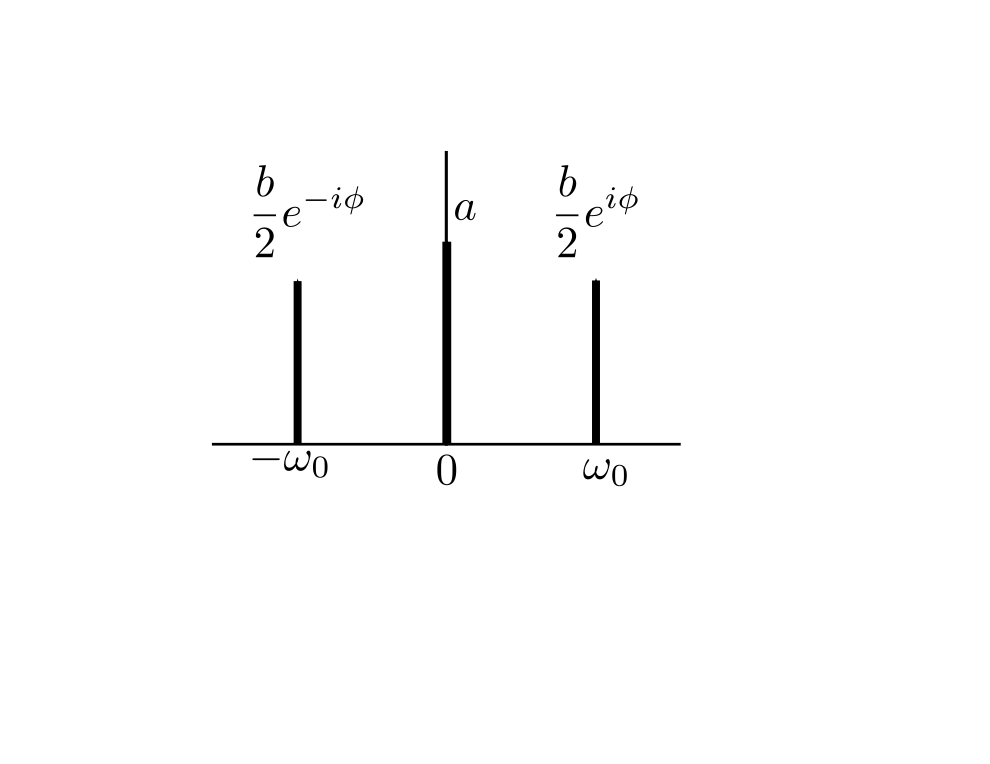
\includegraphics[scale=0.6]{Images/FourierDomine1.png}

\end{center}
\end{frame}
%%%%%%%%%%%%%%%%%%%%%%%%%%%%
\begin{frame}{Algoritos de Cuadratura}
\begin{center}

  \begin{equation}
            H(-\omega_0) =H(0) = 0, H(\omega_0) \neq 0
  \end{equation}
  \includegraphics[scale=0.6]{Images/FourierDomine2.png} 

\end{center}
\end{frame}
%%%%%%%%%%%%%%%%%%%%%%%%%%%%
\begin{frame}{Algoritos de Cuadratura}
\begin{center}

    \begin{equation}
             I(\omega) H(\omega) = \frac{b}{2}exp[i \phi]
     \end{equation}
     \includegraphics[scale=0.6]{Images/FourierDomine3.png}

  \end{center}
\end{frame}
%%%%%%%%%%%%%%%%%%%%%%%%%%%%
\begin{frame}{Algoritmos de Cuadratura}
\begin{center}

  \begin{equation}
    \hat \phi=atan\bigg[ \frac{ Im\{\frac{b}{2}exp[i \phi]\} }{
      Re\{\frac{b}{2}exp[i \phi]\} } \bigg]
  \end{equation}
  \includegraphics[scale=0.6]{Images/wPhase.pdf}

\end{center}
\end{frame}
%%%%%%%%%%%%%%%%%%%%%%%%%%%%
\begin{frame}{Filtros Regularizados}
\begin{center}

\begin{eqnarray}
  U[f(x,y)] &=&\iint_{(x,y) \in S} \Bigg\{ [f(x,y)-I(x,y)]^2 +  \nonumber \\
     & & \eta \bigg[  \frac{\partial f(x,y)}{\partial x} \bigg]^2 +
            \eta \bigg[  \frac{\partial f(x,y)}{\partial y} \bigg]^2 
     \Bigg\} dx dy
\end{eqnarray}
\includegraphics[scale=0.6]{Images/RegularizadosResorte.png}

\end{center}
\end{frame}
%%%%%%%%%%%%%%%%%%%%%%%%%%%%
\begin{frame}{Filtros Regularizados}
\begin{center}

\begin{eqnarray}
  U[f(x,y)] &=&\iint_{(x,y) \in S} \Bigg\{ [f(x,y)-I(x,y)]^2 + 
     \eta \bigg[  \frac{\partial ^2 f(x,y)}{\partial x^2} \bigg]^2 +
                \nonumber \\
      & &\eta \bigg[  \frac{\partial ^2 f(x,y)}{\partial y^2} \bigg]^2 +
     \eta \bigg[  \frac{\partial ^2 f(x,y)}{\partial x \partial y} \bigg]^2
     \Bigg\} dx dy
\end{eqnarray}
\includegraphics[scale=0.6]{Images/RegularizadosPlaca.png}

\end{center}
\end{frame}
%%%%%%%%%%%%%%%%%%%%%%%%%%%%
\begin{frame}{Filtros Regularizados}
\begin{center}

\begin{equation}
  U[f(x,y)]= \sum_{(x,y) \in S} \Big\{  [ f(x,y)-I(x,y) ]^2 + \eta R[f(x,y)] \Big\} 
\end{equation}
Resorte:
\begin{equation}
  R_r [f(x,y)] = [f(x,y)-f(x-1,y)]^2 + [f(x,y)-f(x,y-1)]^2 
\end{equation}

Placa:
\begin{eqnarray}
  R_p [f(x,y)] & = & [f(x+1,y)-2f(x,y)-f(x-1,y)]^2 \nonumber \\
  & & + [f(x,y+1)-2f(x,y)-f(x,y-1)]^2 \nonumber \\
  & & + [ f(x+1,y+1)-f(x-1,y-1) \nonumber \\ 
  & & + f(x-1,y+1)-f(x+1,y-1) ]^2
\end{eqnarray}

\end{center}
\end{frame}
%%%%%%%%%%%%%%%%%%%%%%%%%%%%
\begin{frame}{Filtros Regularizados}
\begin{center}

Resorte:\\
\includegraphics[scale=0.6]{Images/FrecuenciaResorte.png}

\end{center}
\end{frame}
%%%%%%%%%%%%%%%%%%%%%%%%%%%%
\begin{frame}{Filtros Regularizados}
\begin{center}

Placa:\\
\includegraphics[scale=0.6]{Images/FrecuenciaPlaca.png}

\end{center}
\end{frame}
%%%%%%%%%%%%%%%%%%%%%%%%%%%%
\begin{frame}{Filtros Regularizados}
\begin{center}

Resorte 3D:\\
\includegraphics[scale=0.6]{Images/FrecuenciaResorte3D.png}

\end{center}
\end{frame}
%%%%%%%%%%%%%%%%%%%%%%%%%%%%
\begin{frame}{Filtros Regularizados}
\begin{center}

Placa 3D:\\
\includegraphics[scale=0.6]{Images/FrecuenciaPlaca3D.png}

\end{center}
\end{frame}
%%%%%%%%%%%%%%%%%%%%%%%%%%%%
\begin{frame}{Minimos Cuadrados Regularizados}
\begin{center}

\begin{eqnarray}
  I(x,y,k) &=& a(x,y) + b(x,y)\cos[\phi(x,y) +\alpha k] \nonumber \\
  &=& a(x,y) + C(x,y)\cos[\alpha k] - S(x,y)\sin[\alpha k],
\end{eqnarray}
donde:\\
$C(x,y)=b(x,y)\cos[\phi(x,y)]$ \\ 
$S(x,y)=b(x,y)\sin[\phi(x,y)]$

Funcional de minimos cuadrados:
\begin{align}
  U[a,c,s]= \sum_{k=0}^{N-1}\left[a + C \cos(\alpha k)\right.
  -\left. S \sin(\alpha k)-I(k) \right]^2,
\end{align}


\end{center}
\end{frame}
%%%%%%%%%%%%%%%%%%%%%%%%%%%%
\begin{frame}{Minimos Cuadrados Regularizados}
\begin{center}

Funcional de minimos cuadrados regularizados:
\begin{small}
\begin{align}
  U(\bf{a,C,S})=\nonumber\\
  &\sum_{k=0}^{N-1} \sum_{x,y\in L} \left[a + 
  C\cos(\alpha k)\right.
  -\left. S\sin(\alpha k)-I_k \right]^2 M_{x,y}\nonumber \\
  &+\lambda\sum_{x,y\in L}
  \left[(C_{x,y}-C_{x-1,y})^2+(S_{x,y}-S_{x,y-1})^2\right]
  \nonumber\\
  &+\mu\sum_{x,y\in L}(a_{x,y}-a_{x-1,y})^2,
  \label{eq:psi regularized}
\end{align}
\end{small}


\end{center}
\end{frame}
%%%%%%%%%%%%%%%%%%%%%%%%%%%%
\begin{frame}{Minimos Cuadrados Regularizados}
\begin{center}

\includegraphics[scale=0.28]{Images/InterferogramLS.png}\\
\includegraphics[scale=0.28]{Images/LS-Regularized.png}

\end{center}
\end{frame}
%%%%%%%%%%%%%%%%%%%%%%%%%%%%
\begin{frame}{Minimos Cuadrados Regularizados}
\begin{center}

\includegraphics[scale=0.3]{Images/InterferogramLS-exp.png}\\
\includegraphics[scale=0.3]{Images/LS-Regularized-exp.png}

\end{center}
\end{frame}
%%%%%%%%%%%%%%%%%%%%%%%%%%%%
\begin{frame}{Minimos Cuadrados Regularizados}
\begin{center}

Conclusiones!!

\end{center}
\end{frame}
%%%%%%%%%%%%%%%%%%%%%%%%%%%%
\begin{frame}{Self-tuning Regularizados}
\begin{center}

\begin{equation}
I_{k}^{'}(x,y)=b^{'}(x,y)cos(\phi(x,y)+\alpha_{k}),\: k=0,1,2,...,N-1.
\end{equation}

\begin{eqnarray}
U(\bf{f,\alpha}) & = &\sum_{k=0}^{N-1}
\sum_{(x,y)}[\frac{1}{2}[f(x,y)e^{i\alpha_{k}}+f^{*}(x,y)e^{-i\alpha_{k}}]-I_{k}
^{'}(x,y)]^{2}\label{eq:U}\nonumber \\
 &  & +\lambda\sum_{(x,y)}[||D_{x}[f(x,y)]||^{2}+||D_{y}[f(x,y)]||^{2}],\nonumber 
\end{eqnarray}

\end{center}
\end{frame}
%%%%%%%%%%%%%%%%%%%%%%%%%%%%
\begin{frame}{Adaptive phase-shifting}
\begin{center}

\begin{equation}
  I_k(x,y) = a(x,y)+b(x,y)cos[\phi_0(x,y) + \eta_k(x,y) + \omega_0 k],
\end{equation}

renombrando $\beta_k(x,y) = \eta_k(x,y) + \omega_0 k$
\begin{equation}
  I_k(x,y) = a(x,y)+b(x,y)cos[\phi_0(x,y) + \beta_k(x,y)],
\end{equation}


\end{center}
\end{frame}

%%%%%%%%%%%%%%%%%%%%%%%%%%%%
\begin{frame}{Adaptive phase-shifting }
\begin{center}

\begin{equation*}
  E[a(x,y),f(x,y)]=\sum_{k=0}^{K-1}[a(x,y) + Re\{f(x,y) e^{i\beta_k (x,y)} \} -
I_k (x,y)]^2
\end{equation*}

\footnotesize{
\begin{multline*}
\left(\begin{array}{ccc}
K & \sum c_{k}(x,y) & \sum s_{k}(x,y)\\
\sum c_{k}(x,y) & \sum c_{k}(x,y)^{2} & \sum c_{k}(x,y)s_{k}(x,y)\\
\sum s_{k}(x,y) & \sum c_{k}(x,y)s_{k}(x,y) & \sum s_{k}(x,y)^{2}
\end{array}\right)\left(\begin{array}{c}
\hat{a}(x,y)\\
\hat{\phi}(x,y)\\
\hat{\psi}(x,y)
\end{array}\right) = \\ \left(\begin{array}{c}
\sum I_{k}(x,y)\\
\sum I_{k}(x,y)C_{k}(x,y)\\
\sum I_{k}(x,y)S_{k}(x,y)
\end{array}\right)
\end{multline*}
}
\end{center}
\end{frame}
%%%%%%%%%%%%%%%%%%%%%%%%%%%%
\begin{frame}{Adaptive phase-shifting}
\begin{center}

\begin{multline*}
E[a(x,y),g_{k}(x,y)]= \\ \sum_{m=0}^{M-1}\sum_{n=0}^{N-1}\Bigg[\{a(m,n)+Re\{g_{k}(m,
n)e^ { i\phi_{0}(x,y)}\}-I_{k}(m,n)\}h(x-m,y-n)\Bigg]^{2}
\end{multline*}
\begin{multline*}
 \left(\begin{array}{ccc}
[1s*h](x,y) & [\phi*h](x,y) & [\psi*h](x,y)\\{}
[\phi*h](x,y) & [\phi*h]^{2}(x,y) & [\phi\psi*h](x,y)\\{}
[\psi*h](x,y) & [\phi\psi*h](x,y) & [\psi*h]^{2}(x,y)
\end{array}\right)\left(\begin{array}{c}
\hat{a}(x,y)\\
\hat{c}_{k}(x,y)\\
\hat{s}_{k}(x,y)
\end{array}\right)= \\ \left(\begin{array}{c}
[I_{k}*h](x,y)\\{}
[I_{k}\phi*h](x,y)\\{}
[I_{k}\psi*h](x,y)
\end{array}\right)
\end{multline*}


\end{center}
\end{frame}
%%%%%%%%%%%%%%%%%%%%%%%%%%%%
\begin{frame}{Phase Detuning Correcting Method}
\begin{center}

\begin{eqnarray*}
U(f) &=& \sum_{x,y\in L} \mid f(x,y) - g(x,y) \mid ^2 \nonumber\\
      &  &+ \lambda \sum_{x,y\in L} 
  \mid f(x,y) - f(x-1,y) e^{i u_{x,y}} \mid^2 \nonumber\\
  & & + \lambda \sum_{x,y\in L} \mid f(x,y) - f(x,y-1) e^{i v_{x,y}} \mid^2
\end{eqnarray*}
Para $g(x,y)= e^{i \phi^\varepsilon_{x,y}}$

\end{center}
\end{frame}
%%%%%%%%%%%%%%%%%%%%%%%%%%%%
\begin{frame}{Phase Detuning Correcting Method}
\begin{center}

\begin{equation*}
  \nabla \phi_{x,y} = \nabla \left[ \arctan \left(\frac{\sin{\phi_{x,y}}}	
      {\cos{\phi_{x,y}}}\right)\right]
\end{equation*}

\begin{eqnarray*}
  u_{x,y} = \frac{\sin \phi \frac{\partial}{\partial x}  \cos \phi - \cos 
  \phi \frac{\partial}{\partial x} \sin \phi}{ \cos^2 \phi + \sin^2 \phi }
\end{eqnarray*}

\begin{equation*}
  \frac{\partial}{\partial x} \cos\phi_{x,y} = 
  \cos\phi_{x,y}-\cos\phi_{x+1,y},
\end{equation*}

\end{center}
\end{frame}
%%%%%%%%%%%%%%%%%%%%%%%%%%%%
\begin{frame}{Phase Detuning Correcting Method}
\begin{center}

\begin{equation*}
  \nabla \phi_{x,y} = \nabla \left[ \arctan \left(\frac{\sin{\phi_{x,y}}}	
      {\cos{\phi_{x,y}}}\right)\right]
\end{equation*}

\begin{eqnarray*}
  u_{x,y} = \frac{\sin \phi \frac{\partial}{\partial x}  \cos \phi - \cos 
  \phi \frac{\partial}{\partial x} \sin \phi}{ \cos^2 \phi + \sin^2 \phi }
\end{eqnarray*}

\begin{equation*}
  \frac{\partial}{\partial y} \sin\phi_{x,y} = 
  \sin\phi_{x,y}-\sin\phi_{x,y+1}.
\end{equation*}

\end{center}
\end{frame}

%%%%%%%%%%%%%%%%%%%%%%%%%%%%
\end{document}